%
% Documento: Proposta
%


%\chapter{Proposta e Resultados Preliminares}\label{chap:proposta}  
\chapter{Carona solidária para Unifap}\label{chap:Carona solidária para Unifap}  

\section{Perfil da comunidade acadêmica e os problema enfrentados}

Na pesquisa realizada para o projeto entre os meses 05/2019 à 11/2019, os entrevistados (comunidade acadêmica) responderam a seguinte pergunta: \textit{“Qual(is) os motivos já fez(fizeram) você deixar de ir à Universidade?”} e colocamos como opção alguns motivos que podem ter sido os causados, \textit{“Por falta de dinheiro”}, \textit{“Por problemas com chuva”, "Por problemas com o transporte público”}, \textit{“Deslocamento difícil entre casa e Universidade”}, e tivemos como o maior motivo o \textit{“Problemas com o transporte público”}, é possível ver isso na Figura~\ref{fig:dadosmeiodetransporte}%
	%\mnote{Patrícia: as figuras serão citadas assim, usando o label que foi definido em cada uma delas. Assim se atualiza sozinho o número de cada uma.}
    %.
%
	%\mnote{Patrícia: melhorar o título das figuras, tem que dizer mais sobre o que elas representam.}
    % comentado para não aparecer no compilado
\begin{figure}[!hbtp]
	\centering
	\caption{Pergunta sobre os motivos que fizeram os alunos não comparecerem a universidade.}
	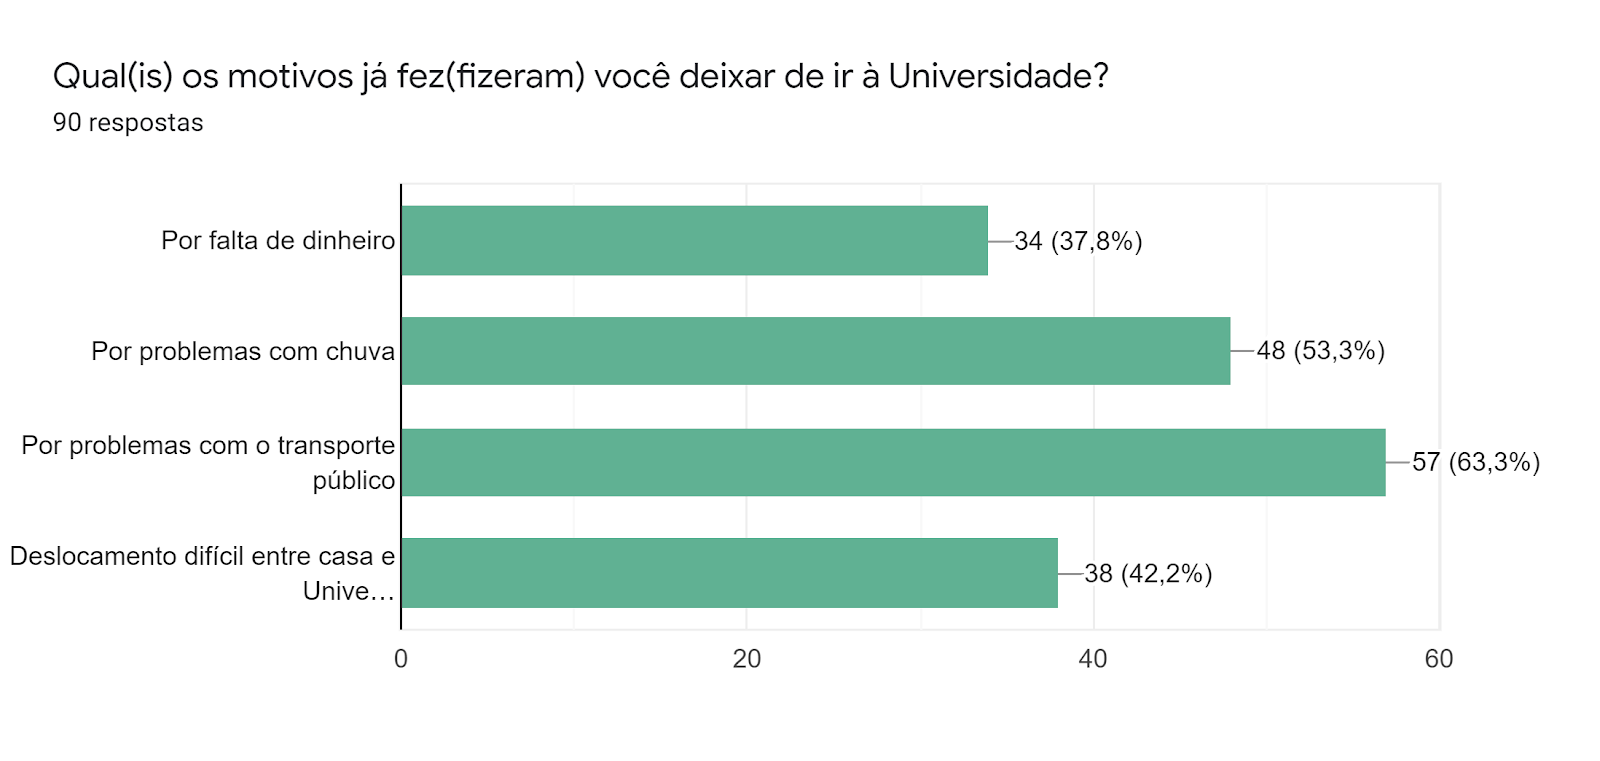
\includegraphics[width=0.8\textwidth]{./04-figuras/questionario/1.png}
	\label{fig:dadosmeiodetransporte}
	\fonte{Elaborado pelo autor.}
\end{figure}

Proveniente disso, hoje já existem reflexos de problemas relacionados à mobilidade, meio ambiente, economia, etc., e motivado por isso, que será proposto uma solução relacionada à mobilidade inicialmente.

%Pensando nisso, foi observado que existe uma necessidade de melhorias em relação ao acessos dos alunos a universidade ....

%\section{Resultados do questionário}

Foi elaborado um questionário com 16 perguntas e obteve 186 respostas, com o objetivo de saber mais sobre a comunidade acadêmica, entre elas, perguntas sobre o sexo, se possui veículo, em qual período que frequenta a universidade, e quantidade de dias que frequenta, todas para entender melhor o perfil e a possibilidade do projeto se encaixar no ambiente universitário, como mostra a \ref{fig:genero}.

\begin{figure}[!hbtp]
	\centering
	\caption{Gênero dos entrevistados}
	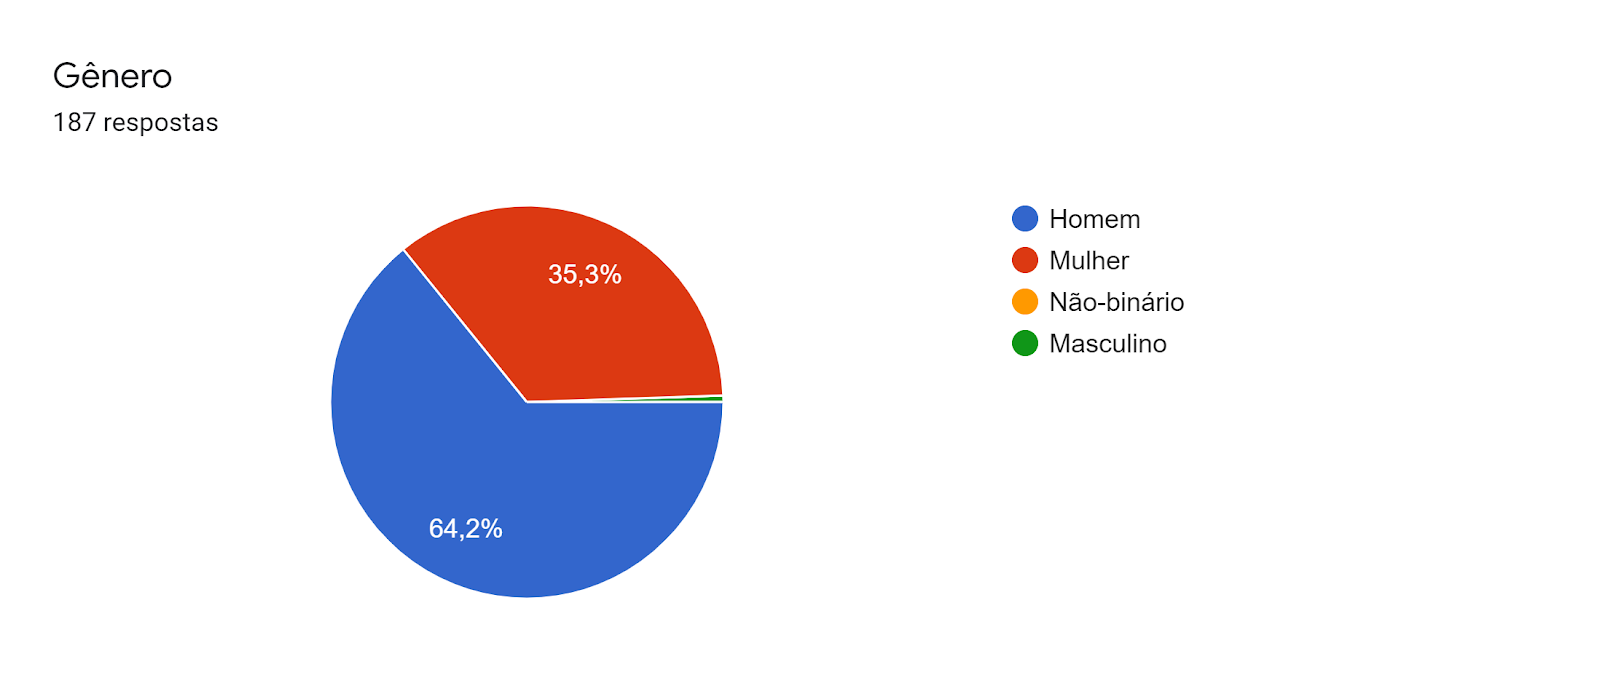
\includegraphics[width=0.8\textwidth]{./04-figuras/questionario/2.png}
	\label{fig:genero}
	\fonte{Elaborado pelo autor.}
\end{figure}

Foi possível verificar, analisando os resultados do questionário, quais seriam os empecilhos a adesão do projeto, e há uma rejeição em relação a segurança do transporte, principalmente pelas mulheres, que fazem parte de 35,3\% dos entrevistados, possível ver isso na Figura~\ref{fig:aceitacaopelascaronas} e Figura~\ref{fig:aceitacaopelascaronas2}%.

\begin{figure}[!hbtp]
	\centering
	\caption{Motivo para aceitar as caronas - Parte 1}
	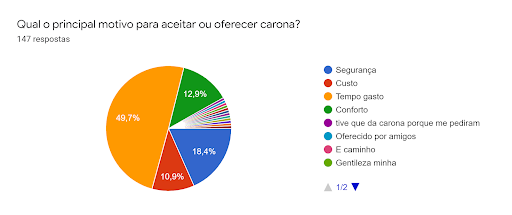
\includegraphics[width=0.7\textwidth]{./04-figuras/questionario/3.png}
	\label{fig:aceitacaopelascaronas}
	\fonte{Elaborado pelo autor.}
\end{figure}

\begin{figure}[!hbtp]
	\centering
	\caption{Motivos para aceitar as caronas - Parte 2}
	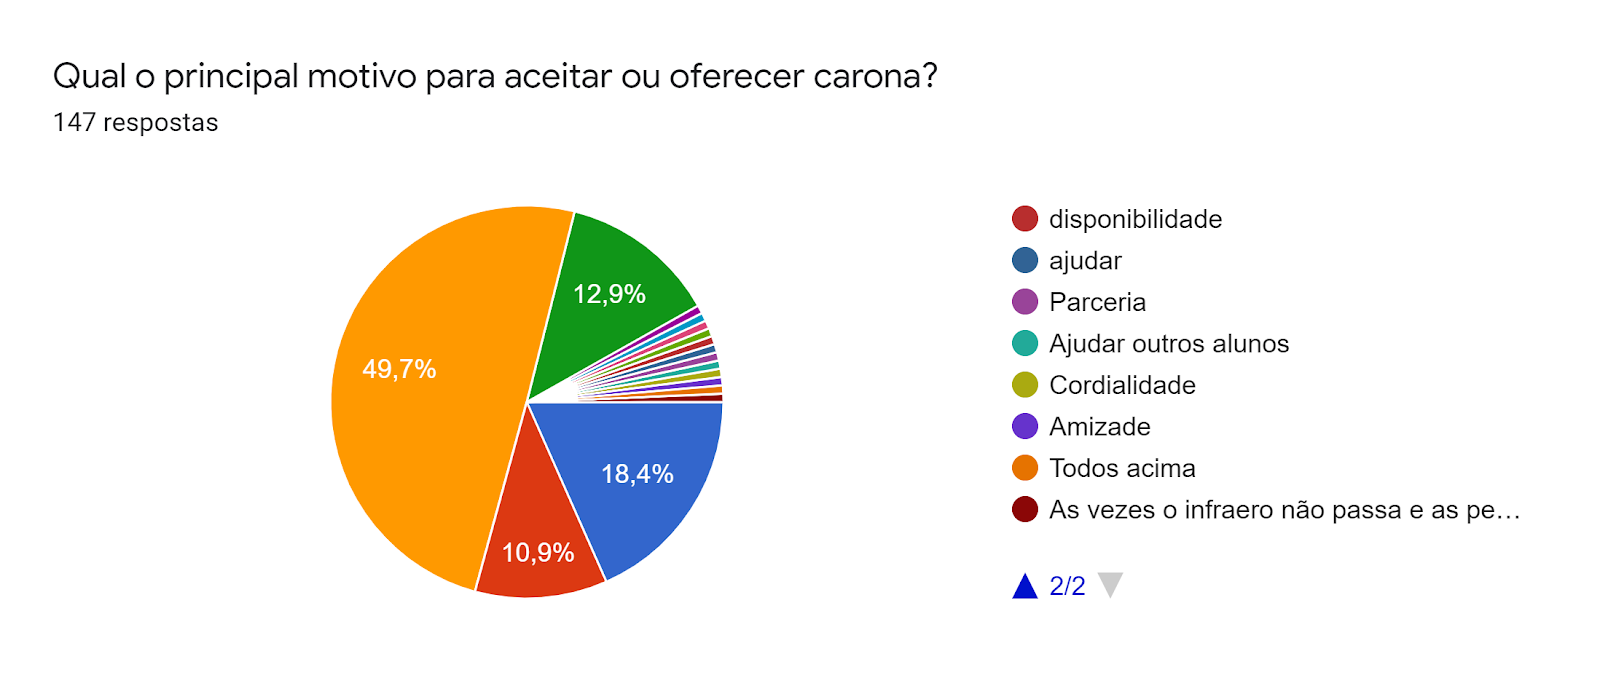
\includegraphics[width=0.7\textwidth]{./04-figuras/questionario/4.png}
	\label{fig:aceitacaopelascaronas2}
	\fonte{Elaborado pelo autor.}
\end{figure}

Outros motivos mencionados nesta pergunta foram, \textit{“não ter alguém para oferecer”}, \textit{“falta de oportunidade”}, \textit{“não conheço nenhum aplicativo de carona, motivos que demonstram o interesse da comunidade de receber/oferecer caronas."}

Pensando nisso, para obter um resultado satisfatório para todos, é pensado algo que foi utilizado em outros projetos relacionados a carona solidária por outras universidades, que é ter como usuários, as pessoas que tem um vínculo ativo com a instituição, utilizando a base de acesso ao sistema da universidade, podendo haver tanto alunos, professores e técnicos como usuários.

Quando questionados sobre essa opção, o projeto teve uma grande aceitação por parte da comunidade acadêmica, Figura~\ref{fig:aceitacao}.%

\begin{figure}[!hbtp]
	\centering
	\caption{Pergunta sobre a possibilidade da proposta ser utilizada apenas por pessoas da Unifap}
	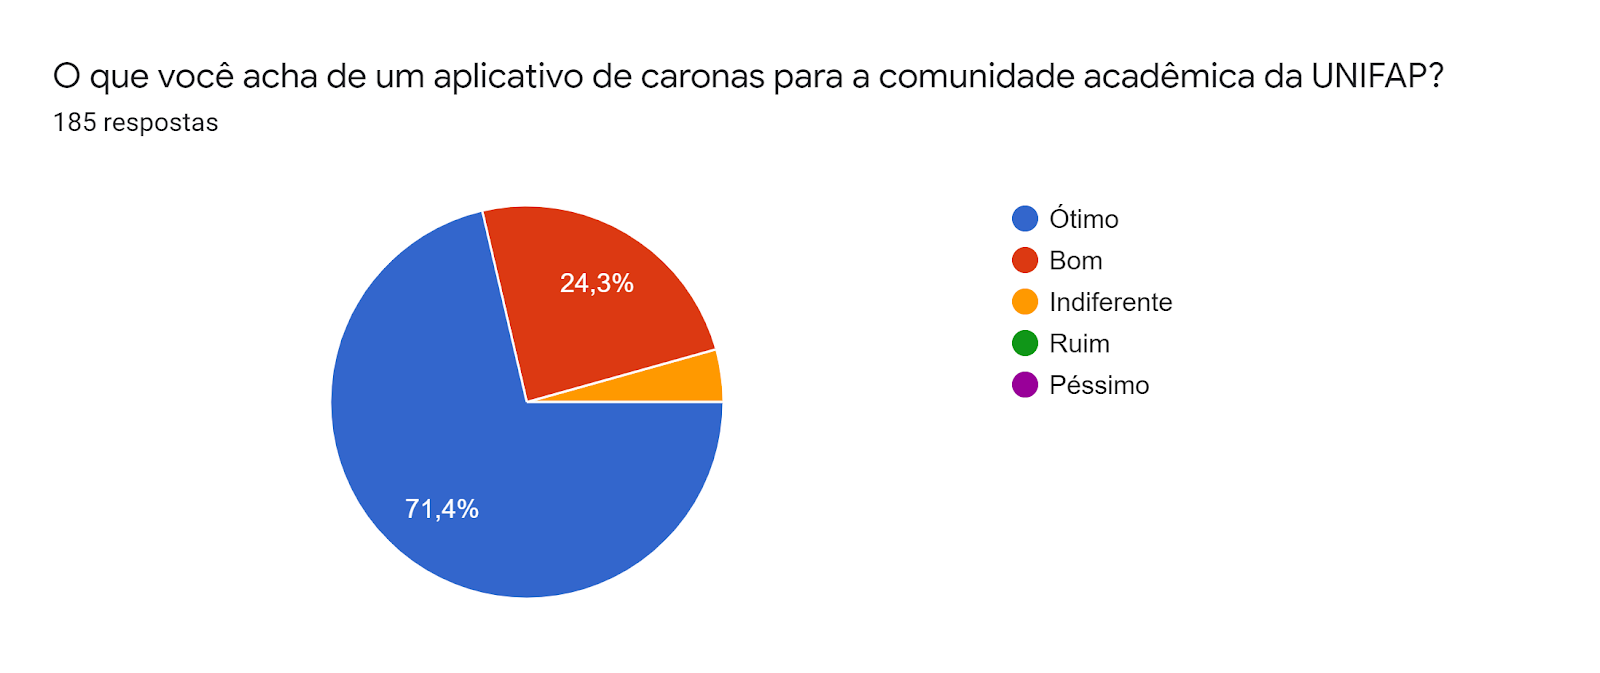
\includegraphics[width=0.7\textwidth]{./04-figuras/questionario/5.png}
	\label{fig:aceitacao}
	\fonte{Elaborado pelo autor.}
\end{figure}

Pensando no aspecto cultural, será realizado campanhas para incentivar e popularizar o projeto por meio de cartazes espalhados pela universidade, e para melhorar o encontro entre os “caroneiros”, existe a possibilidade de criar pontos de encontros para facilitar mais a vida de quem está disposto a oferecer a carona.

A pesquisa deu-se pela pesquisa bibliográfica, estudo de caso e um levantamento de dados por um questionário utilizando a plataforma Google Forms, compreendeu-se que um sistema de caronas para a universidade iria melhorar as condições de mobilidade da instituição e dar outra alternativa ao membro da comunidade acadêmica.

Para muitos, o transporte para ir e vir à universidade se torna o grande problema durante a vida acadêmica, tomando um tempo destes para chegar a Universidade e para retornar às suas casas durante os dias letivos, tendo grande espera nas paradas de ônibus, tempo que poderia ser aproveitado para estudar. Mais de 50\% dos entrevistados do formulário responderam que estão insatisfeitos com o transporte que utilizam, isso é apresentado na Figura~\ref{fig:satisfacao}.

\begin{figure}[!hbtp]
	\centering
	\caption{Pergunta sobre a satisfação dos usuários com o transporte que utiliza}
	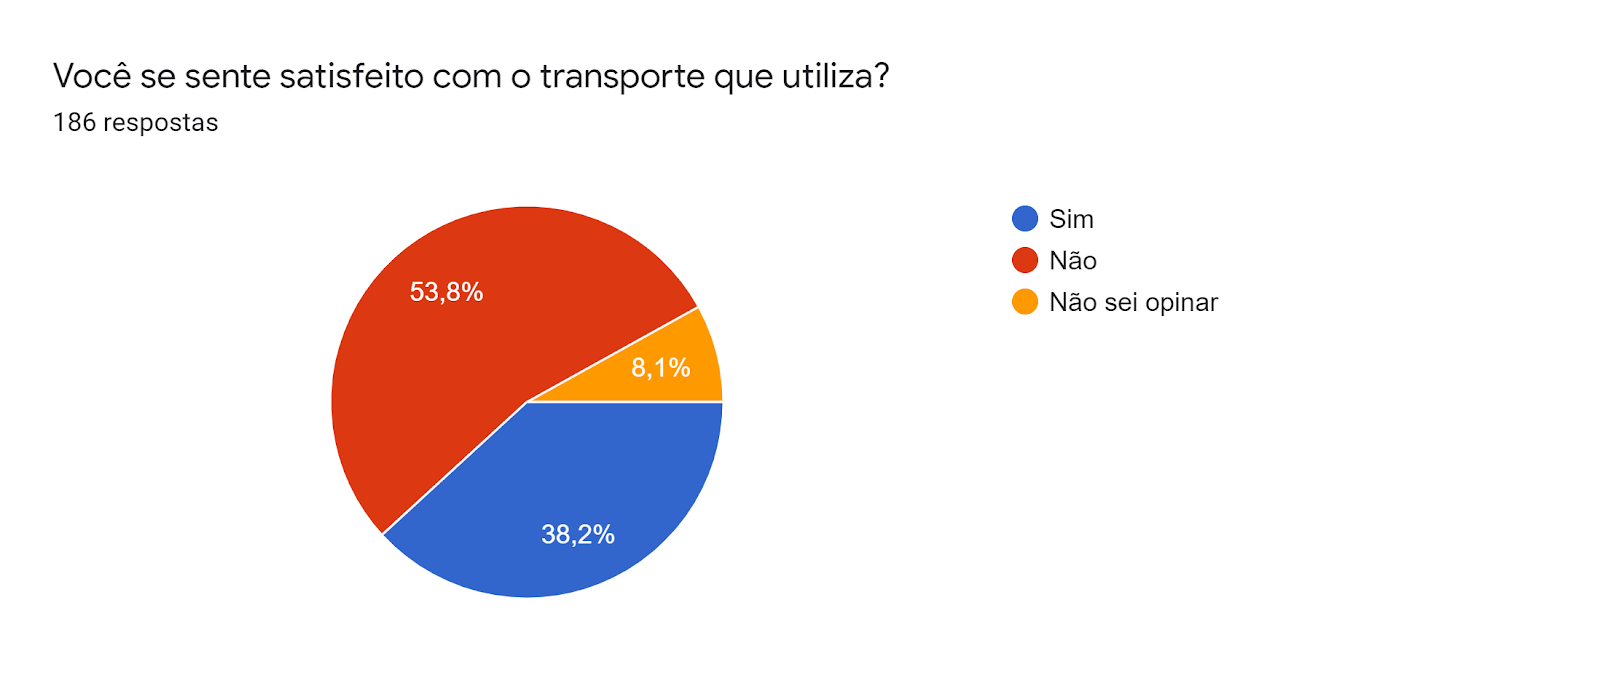
\includegraphics[width=0.7\textwidth]{./04-figuras/questionario/6.png}
	\label{fig:satisfacao}
	\fonte{Elaborado pelo autor.}
\end{figure}

E mais de 50\% destes entrevistados utilizam o transporte público para chegar ou sair da Universidade, e nessa mesma pergunta conseguimos estimar a quantidade dos entrevistados que possuem carro próprio, 26,9\% responderam que utilizam carro para chegar a universidade e 24,7\% utilizam para sair da Universidade, como mostra a figura \ref{fig:chegadanaunifap1} e \ref{fig:saidadaunifap1}.

\begin{figure}[!hbtp]
	\centering
	\caption{Como você geralmente chega na Unifap? -  Parte 1}
	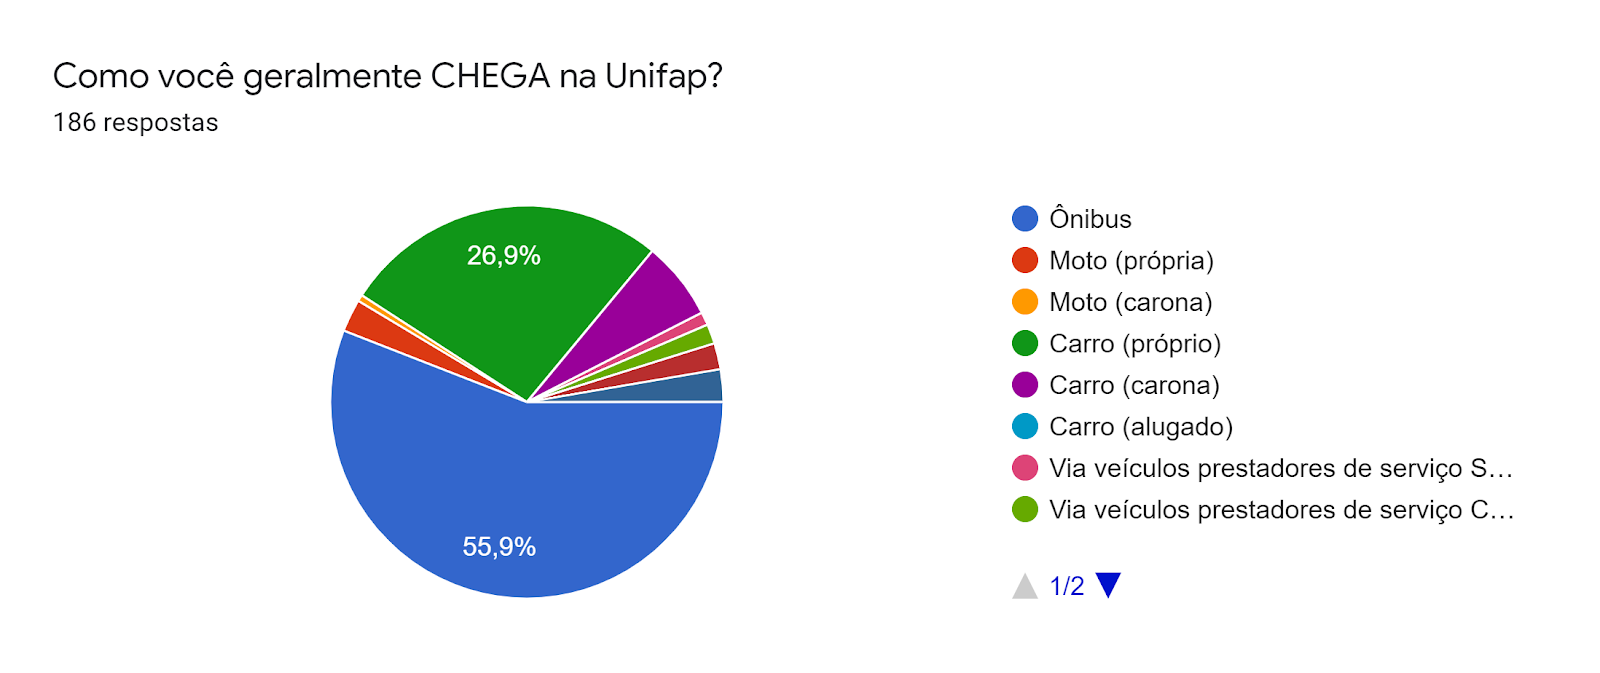
\includegraphics[width=0.6\textwidth]{./04-figuras/questionario/7.png}
	\label{fig:chegadanaunifap1}
	\fonte{Elaborado pelo autor.}
\end{figure}

\begin{comment}
\begin{figure}[!hbtp]
\centering
\caption{Como você geralmente chega na Unifap? - Parte 2}
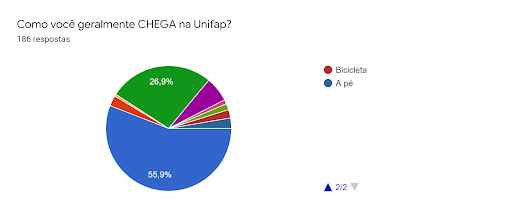
\includegraphics[width=0.6\textwidth]{./04-figuras/questionario/8.png}
\label{fig:chegadanaunifap2}
\fonte{Elaborado pelo autor.}
\end{figure}
\end{comment}


\begin{figure}[!hbtp]
	\centering
	\caption{Como você geralmente sai da Unifap? - Parte 1}
	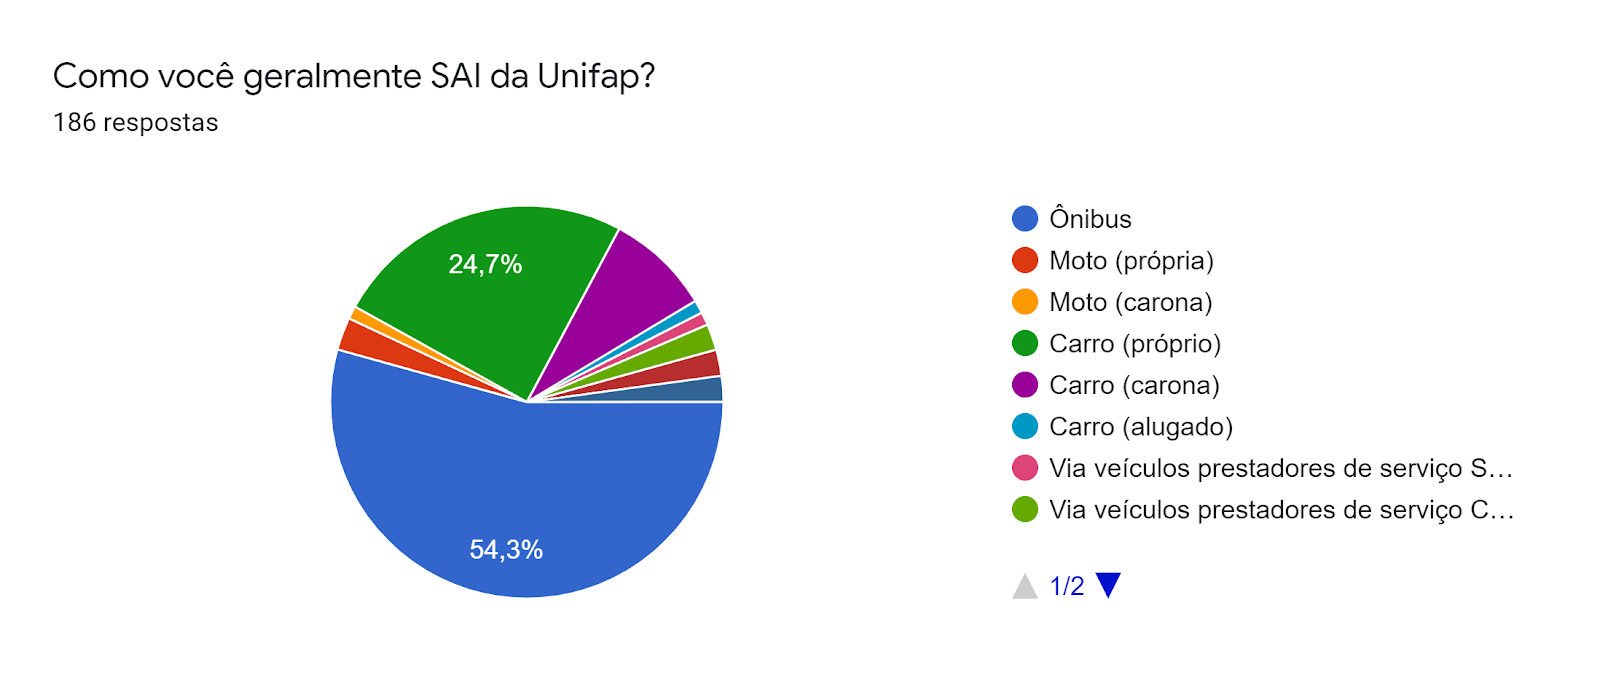
\includegraphics[width=0.6\textwidth]{./04-figuras/questionario/9.png}
	\label{fig:saidadaunifap1}
	\fonte{Elaborado pelo autor.}
\end{figure}

\begin{comment}
	conteúdo...\begin{figure}[!hbtp]
	\centering
	\caption{Como você geralmente sai da Unifap - Parte 2}
	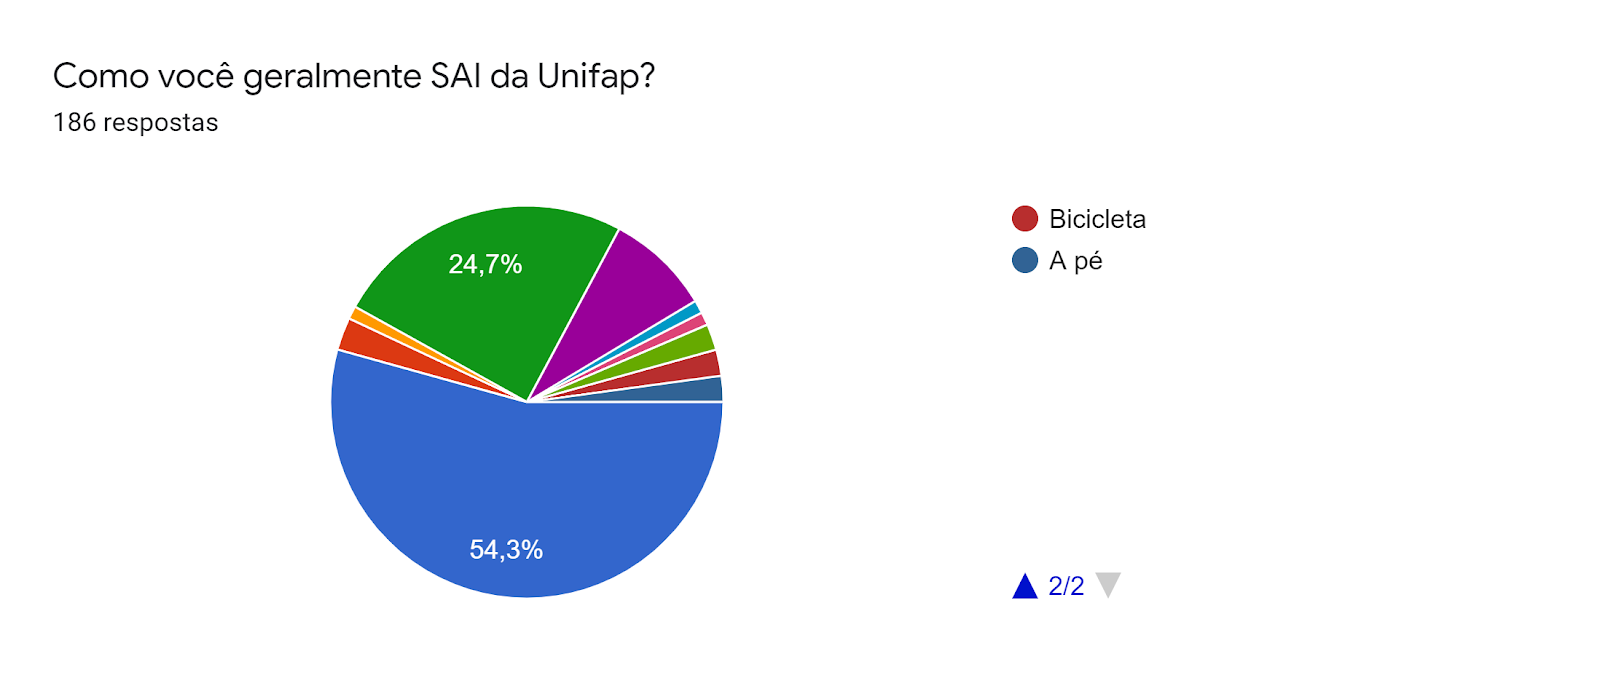
\includegraphics[width=0.6\textwidth]{./04-figuras/questionario/10.png}
	\label{saidadaunifap2}
	\fonte{Elaborado pelo autor.}
	\end{figure}
\end{comment}



As condições insatisfatórias do sistema de transporte local, além das demoras, superlotação e conforto, os acadêmicos ainda ficam expostos à criminalidade, muitas vezes esperando em paradas escuras durante o período noturno.

A maior parte dos acadêmicos apontam como principais problemas, a segurança, o tempo gasto e o conforto que na pesquisa é de suma importância durante o trajeto de ida e volta da universidade. Dos 100 entrevistados que responderam a esta pergunta, 75\% apontam o conforto como um dos problemas, como mostra na figura \ref{fig:problemasenfrentadosparair}.

\begin{figure}[!hbtp]
	\centering
	\caption{Principais problemas enfrentados com o transporte público local}
	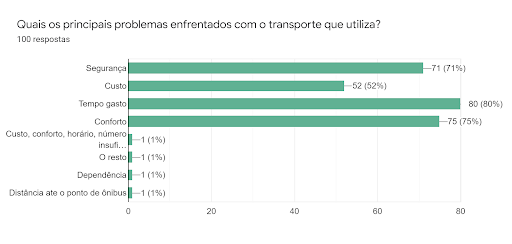
\includegraphics[width=0.6\textwidth]{./04-figuras/questionario/11.png}
	\label{fig:problemasenfrentadosparair}
	\fonte{Elaborado pelo autor.}
\end{figure}


Na figura \ref{fig:motivos-nao-ir-a-unifao}, das 187 respostas ao questionário, 90 respostas, um pouco menos que 50\% dos entrevistados, responderam quais são os motivos que impedem de ir à universidade, e problemas com o transporte público é o de mais da metade dos que responderam o questionário.

\begin{figure}[!hbtp]
	\centering
	\caption{Motivos que já fizeram alunos deixarem de ir a Universidade}
	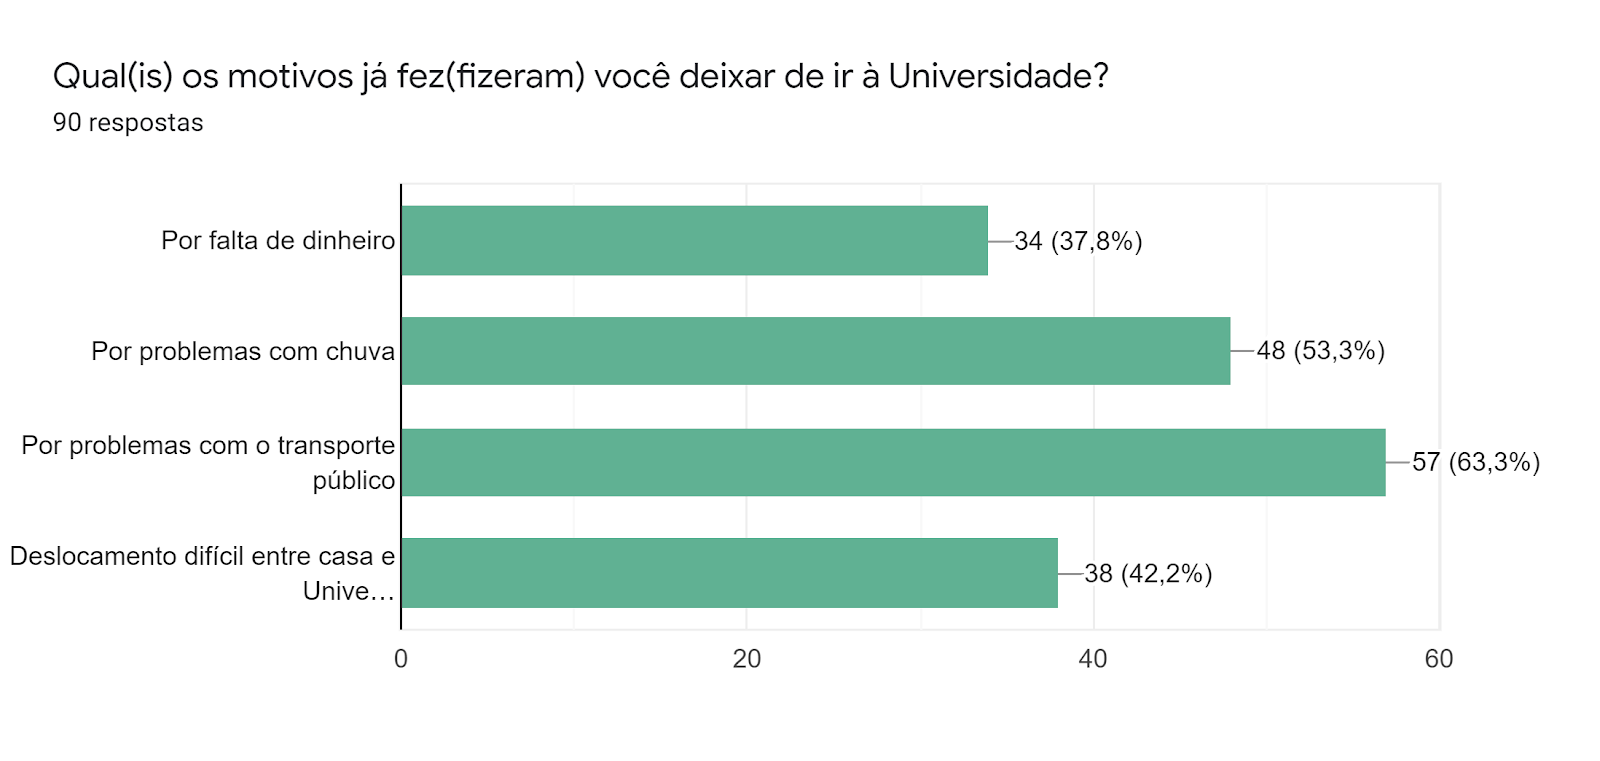
\includegraphics[width=0.6\textwidth]{./04-figuras/questionario/12.png}
	\label{fig:motivos-nao-ir-a-unifao}
	\fonte{Elaborado pelo autor.}
\end{figure}

Sobre as relações com o tempo gasto, não pararam de ser mencionadas, quando perguntados quais os motivos de aderirem um sistema de caronas, a maioria dos entrevistados apontaram também o tempo gasto como motivo para aceitar caronas, dados apresentados nas figuras \ref{fig:motivosparacarona1} e \ref{fig:motivosparacarona2}.

\begin{figure}[!hbtp]
	\centering
	\caption{Motivos para aceitar carona - Parte 1}
	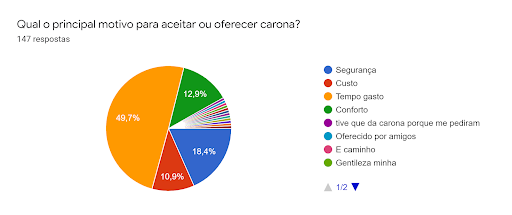
\includegraphics[width=0.7\textwidth]{./04-figuras/questionario/13.png}
	\label{fig:motivosparacarona1}
	\fonte{Elaborado pelo autor.}
\end{figure}

\begin{figure}[!hbtp]
	\centering
	\caption{Motivos para aceitar carona - Parte 2}
	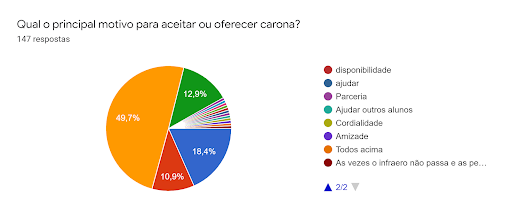
\includegraphics[width=0.7\textwidth]{./04-figuras/questionario/14.png}
	\label{fig:motivosparacarona2}
	\fonte{Elaborado pelo autor.}
\end{figure}

Quando foi perguntado aos entrevistados se participavam de grupos de caronas, 96,6\% responderam à pesquisa que \textit{“Não participavam”}. Então, um aplicativo de caronas para a universidade poderá criar uma cultura que ainda é inexistente.

Das 185 pessoas que responderam o questionário, 97.7\% dos entrevistados acharam \textit{“ótima”} ou \textit{“boa”} a iniciativa de um aplicativo que os usuários possam consultar viagens de ida para a universidade ou de volta da universidade, como mostra na figura \ref{fig:percepcao}.
\begin{figure}[!hbtp]
	\centering
	\caption{Percepção sobre a proposta de um aplicativo de carona para a Unifap}
	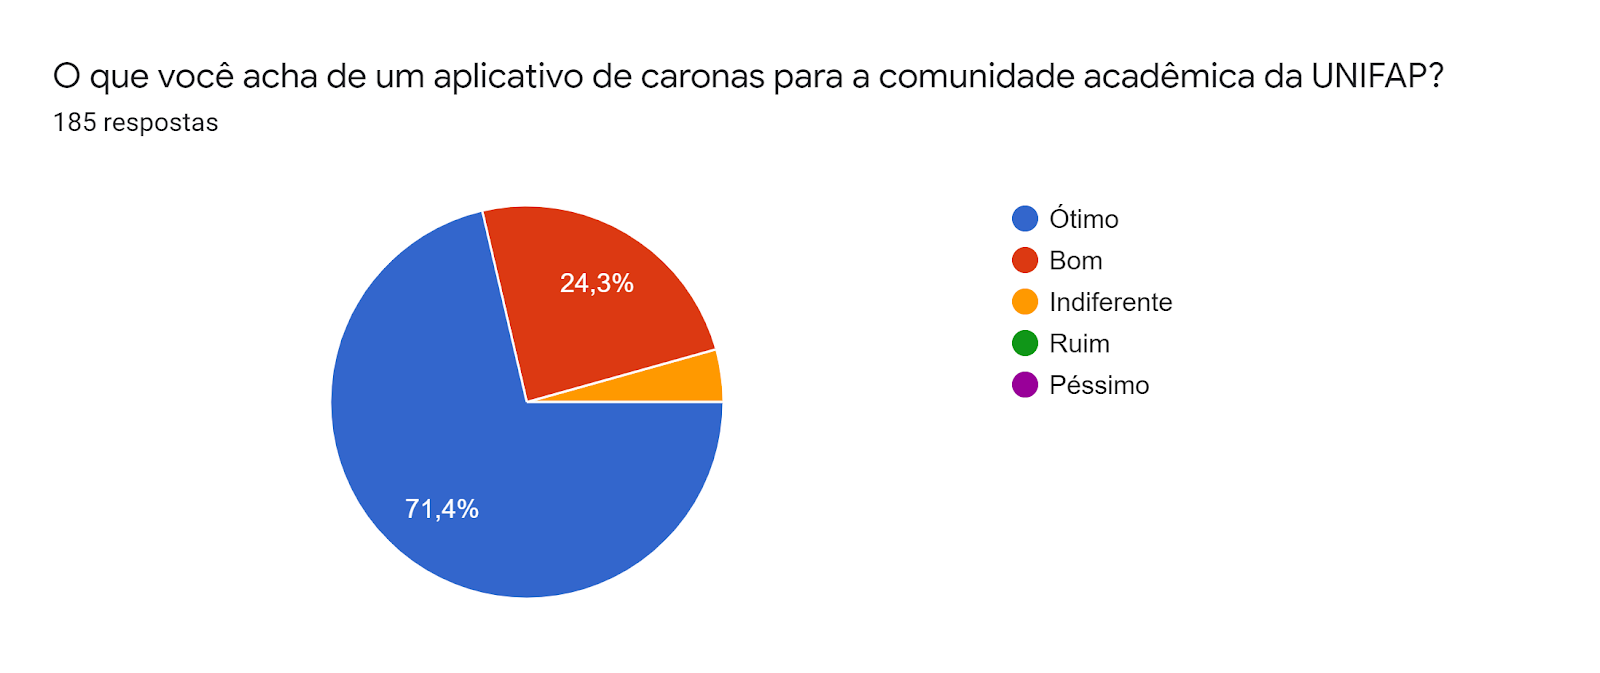
\includegraphics[width=0.7\textwidth]{./04-figuras/questionario/15.png}
	\label{fig:percepcao}
	\fonte{Élaborado pelo autor.}
\end{figure}

Em relação a esse uso de tecnologia, a comunidade acadêmica já está bem familiarizada com aplicativos relacionados à mobilidade, na figura \ref{fig:conhecimento-sobre-apps}, das 186 respostas ao questionário, apenas 15,1\% responderam não utilizar nenhum dos aplicativos listados.

\begin{figure}[!hbtp]
	\centering
	\caption{Percepção sore o conhecimento e uso de tecnologias similares a proposta}
	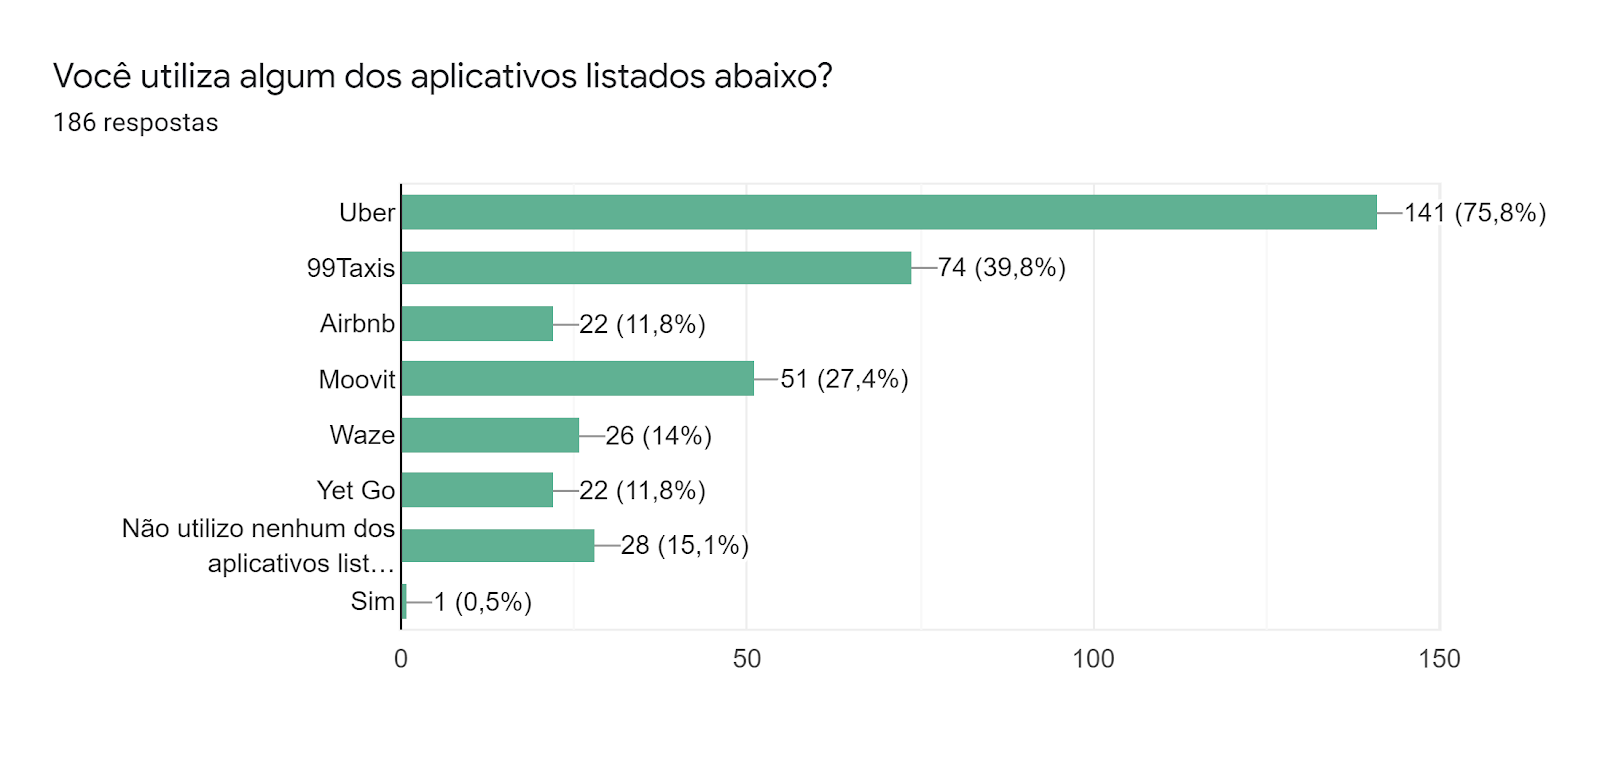
\includegraphics[width=0.7\textwidth]{./04-figuras/questionario/16.png}
	\label{fig:conhecimento-sobre-apps}
	\fonte{Elaborado pelo autor.}
\end{figure}

No questionário, foi verificado o tempo gasto pela comunidade utilizando smartphones, dispositivo necessáriao para o uso do aplicativo, e apenas 1,6\% dos entrevistados informaram que não possuem smartphones, e 37\% passam mais de 6h utilizando os dispositivos diariamente, como mostra na figura \ref{fig:usodosmartphone}.

\begin{figure}[!hbtp]
	\centering
	\caption{Tempo de uso do \textit{Smartphone} pelos entrevistados}
	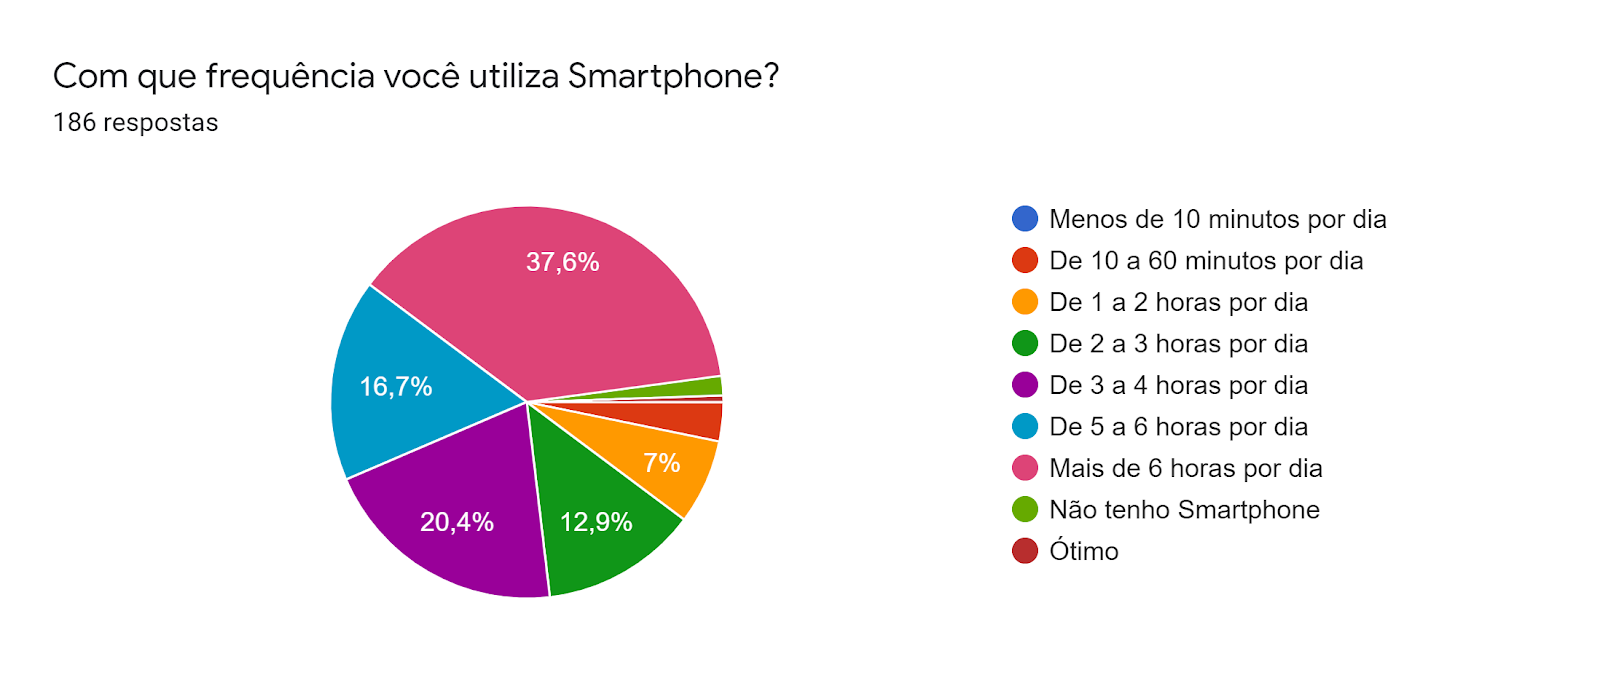
\includegraphics[width=0.7\textwidth]{./04-figuras/questionario/17.png}
	\label{fig:usodosmartphone}
	\fonte{Elaborado pelo autor}
\end{figure}

O resultado foi satisfatório, percebe-se que a comunidade está disposta a aderir a proposta do aplicativo de carona solidária, onde muitos se interessam em oferecer ou receber carona. 
%porém, falta algo que auxilie-os.

\section{Definições dos Requisitos}

Para definirmos os requisitos funcionais e não funcionais da solução, levamos em consideração o questionário realizado, as soluções já existentes e consolidadas e soluções open-source.

Levando em consideração o questionário realizado, o requisito mais importante e de suma importância para o projeto será a funcionalidade da solução ser acessada apenas por pessoas vinculadas a Unifap.

%- Acesso somente a usuários da comunidade acadêmica

%- Viagens de ida e volta da Universidade

%- Aplicativo restrito à comunidade acadêmica

%- Opção de oferecer caronas

%- Opção de aceitar caronas

%- Histórico de carona

\subsection{Requisitos Funcionais}
% COLOCAR TELAS DA APLICAÇÃO
\textbf{[RF001] Login no Sistema}

\textbf{Prioridade}:      [x] Essencial        [] Importante     [] Desejável 

\textbf{Atores}: Motoristas e passageiros


O sistema deve permitir ao discente o acesso solicitando seu CPF e senha dos usuários cadastrados.
%%%%%%%%%%

\textbf{[RF002] Registro de Corrida}

\textbf{Prioridade}:      [x] Essencial        [] Importante     [] Desejável 

\textbf{Atores}: Motoristas e passageiros

O sistema deve permitir ao discente a criação de uma carona informando ponto de saída ou ponto de chegada com a Universidade em um desses 2 pontos.
%%%%%%%%%%%

\textbf{[RF003] Consultar Corridas}

\textbf{Prioridade}:      [] Essencial        [x] Importante     [] Desejável 

\textbf{Atores}: Motoristas e passageiros

O sistema deve permitir ao discente a consulta das corridas catalogadas no sistema, com informações sobre trajeto, motorista, e informações do veículo.

\textbf{[RF004] Detalhe da Corrida}

\textbf{Prioridade}:      [] Essencial        [x] Importante     [] Desejável 

\textbf{Atores}: Motoristas e passageiros

O sistema deve permitir ao discente consulte o detalhe da corrida, cor do veículo, placa, porto de encontro e rota da corrida.

\textbf{[RF005] Criar rotina de corridas}

\textbf{Prioridade}:      [] Essencial        [] Importante     [x] Desejável 

\textbf{Atores}: Motoristas

O sistema deve permitir o usuário que deseja ofertar caronas possa criar a sua rotina de viagens sem que precise diariamente criar suas viagens de ida e de volta.


\textbf{[RF006] Consulta de caronas ofertadas}

\textbf{Prioridade}:      [] Essencial        [] Importante     [x] Desejável 

\textbf{Atores}: Motoristas

O sistema deve permitir o usuário consiga ver as suas caronas ofertadas.


\textbf{[RF007] Consulta de caronas pendentes}

\textbf{Prioridade}:      [] Essencial        [] Importante     [x] Desejável 

\textbf{Atores}: Motoristas e passageiros

O sistema deve permitir os usuários consultarem suas caronas que ainda serão realizadas.


\textbf{[RF008] Consultar perfil}

\textbf{Prioridade}:      [] Essencial        [X] Importante     [] Desejável 

\textbf{Atores}: Motoristas e passageiros

O sistema deve permitir que os usuários de uma carona possam consultar seus perfis, com as informações de nome, c


\textbf{[RF009] Falaê}

\textbf{Prioridade}:      [] Essencial        [X] Importante     [] Desejável 

\textbf{Atores}: Motoristas e passageiros

O sistema deve permitir que os usuários tenham uma forma de se comunicar com os gestores da ferramenta, com críticas, sugestões, elogios

\textbf{[RF010]  Tela de perguntas frequentes}

\textbf{Prioridade}:      [] Essencial        [X] Importante     [] Desejável 

\textbf{Atores}: Motoristas e passageiros

O sistema disponibiliza informações rápidas as dúvidas mais comuns em relação a aplicação.

\textbf{[RF011] Área do Administrador}

\textbf{Prioridade}:      [] Essencial        [X] Importante     [] Desejável 

\textbf{Atores}: Motoristas e passageiros

O sistema deverá permitir que o administrador visualize
estatísticas por meio de uma interface web.

\textbf{[RF012] Concordar com os termos de uso} 

\textbf{Prioridade}:      [] Essencial        [X] Importante     [] Desejável 

\textbf{Atores}: Motoristas e passageiros

Os usuários devem concordar com o termo de uso do aplicativo antes de utilizá-los.


\subsection{Requisitos Não Funcionais}

\textbf{[NF001] O sistema mobile foi desenvolvido na plataforma Android sendo compatível a versão 4.0 ou superior. %Compatibilidade%
}

\textbf{Prioridade}:      [x] Essencial        [] Importante     [] Desejável 

%O sistema mobile foi desenvolvido na plataforma Android sendo compatível a versão 4.0 ou superior.


\textbf{[NF002] O sistema deve estar sempre disponível  aos seus usuários, independente de horário ou dia da semana. %Disponibilidade%
}

\textbf{Prioridade}:      [x] Essencial        [] Importante     [] Desejável 

\textbf{[NF003] O aplicativo deve ser implementado na linguagem Java}


\textbf{Prioridade}:      [x] Essencial        [] Importante     [] Desejável 


%O sistema deve estar sempre disponível online aos seus usuários, independente de horário ou dia da semana.



\textbf{[NF004] O sistema deverá se comunicar com o banco SQL Server}

\textbf{Prioridade}:      [x] Essencial        [] Importante     [] Desejável 












\begin{comment}
\begin{table}[]
\centering
\caption{RF001 Registro de Carona}
\label{tab:rf-001}
\begin{tabular}{l|l|l|l|l|}
\hline
\multicolumn{5}{|l|}{RF001 REGISTRO DE CARONA} \\ \hline
Referência & \multicolumn{4}{l|}{} \\ \cline{2-5} 
Sumário & \multicolumn{4}{l|}{} \\ \cline{2-5} 
Pré-condições & \multicolumn{4}{l|}{} \\ \cline{2-5} 
Atores & \multicolumn{4}{l|}{} \\ \cline{2-5} 
Descrição & \multicolumn{4}{l|}{} \\ \cline{2-5} 
\end{tabular}
\end{table}
\end{comment}


\begin{comment}
\begin{itemize}
    \item O usuário
\end{itemize}
\begin{itemize}
    \item Requisitos do Usuário
    \item Requisitos do Sistema
    \item Requisitos de Negócio
\end{itemize}
\end{comment}

\section{Estudo sobre Soluções de Mobilidade Inteligente}

%PESQUISA DE ACEITAÇÃO DO CARONAE
%TELAS

\begin{comment} %%%%%%%%%%%%%%%%%%%%%%%%%%%%%%%%%%%%%%%%%%%%%%%%%%%%%%%%%%%%%%%%%%%%%%%%%%%%%%%%%
    
	\mnote{Patrícia: aqui vais colocar tuas considerações (sem afirmarnada sem dados e provas) sobre as pesquisas que fizeste feitas em relação a cidades inteligentes e, em especial, mobilidade inteligente. Cita algumas soluções que são utilizadas e vai fazendo considerações do porque elas nao tem como ser consideradas (ainda) para Macapá e para a comunidade acadêmica da Unifap. No final, depois de discutir sobre diferentes soluções fala das soluções de carona e o porquê ela foi considera como a "melhor" opção no momento para Unifap.}
    
\end{comment} %%%%%%%%%%%%%%%%%%%%%%%%%%%%%%%%%%%%%%%%%%%%%%%%%%%%%%%%%%%%%%%%%%%%%%%%%%%%%%%%%%

Após realizar o estudo de algumas das possíveis soluções de mobilidade que podem ser implementadas na Unifap, e analisa-las, chegamos na conclusão que no cenário atual, duas soluções apresentadas seriam possíveis para o cenário atual da Unifap, Uma delas seria o aplicativo Waze Carpool, e a outra o aplicativo de carona solidária Caronaê, solução de código aberto da Universidade Federal do Rio de Janeiro.

As demais soluções foram descartadas por alguma inviabilidade, como exemplo, a solução de compartilharmos bicicletas, semelhante a da startup \textit{Yellow}, termos a \textit{Yellow} não seria possível, a empresa não tem nenhum serviço voltados para o uso restrito, ou a um determinado grupo, caso quiséssemos criar uma solução semelhante, teríamos problemas com a aquisição das bicicletas e locais para guardá-las, além de termos em mãos um transporte que proporcionaria insegurança aos usuários por falta de ciclovia em muitos pontos da cidade.

Pensar em uma ideia de orientação de mobilidade também seria inviável, por termos um serviço de transporte público insuficiente \cite{sau2018}, que não apresenta conformo e já tem muitas reclamações a seu respeito. Seria difícil seguirmos com nossos objetivos e mais os resultados que colhemos com o formulário com essas soluções.

Então, analisamos as opções de solução mais aptas a serem implementadas com o auxílio da tecnologia, foi que encontramos a opção de um aplicativo de carona solidária onde o objetivo é melhorar e dar mais uma opção de meio de transporte a comunidade universitária, mas precisamente o aplicativo de código aberto regido pela GLP-3.0 License, disponível no GitHub.

\subsection{Waze Carpool x Caronaê}
    Durante todo o levantamento das soluções de mobilidade que poderiam ser escolhidas para a proposta do projeto, duas se fizeram mais próximas daquilo que nós gostariamos, são elas, Waze Carpool e o aplicativo Caronaê, ambos são aplicativos de carona.
    
    O Waze Carpool, da empresa Waze tem uma proposta de compartilhar corridas com grupos de amigos, grupos de trabalho, grupos de uma universidade, entre outros grupos que queiram partir da mesma ideia. Da forma que o Waze Carpool organiza as caronas, o motorista que irá oferece a carona utiliza o aplicativo Waze que já é utilizado bastante como uma solução de orientação de mobilidade, e o usuário que quer pegar as caronas precisa baixar o aplicativo Waze Carpool.
    
    As coisas podem ser ofertadas sem restrição, para todos os usuários da sua localidade, ela estará visível para todos, e pode também ser criado grupos. Para entrar nos grupos, que são criados ou pela Waze ou por uma pessoa que fica responsável pelo gerenciamento do grupo, a Waze chama de "embaixador", está pessoa fica encarregada de compartilhar o link ou QR Code de acesso. 
    
    Já o aplicativo Caronaê, surgiu na UFRJ também com a proposta de oferecer caronas aos alunos da Universidade do Rio de Janeiro, mas precisamente, dos Campus do Fundão e da Praia Vermelha. O aplicativo inicialmente era de uso apenas do corpo docente da UFRJ, com características de um catalogo de caronas, o aplicativo oferece características também de um PGV. 
    
    Por ser pensado para um universidade, pensando no conforto, praticidade, e como oferecer segurança ao utilizar o aplicativo, restringindo o uso apenas para alunos, professores e técnicos, o Caronaê, que disponibilizou seu código para outras universidades implementarem a ideia, espalharem o proposito do projeto, da cultura de caronas, da importância de reduzirmos o número de veículos nas ruas, se apresenta junto com o Waze Carpool, boas soluções, porém, o diferencial do Caronaê está justamente na possiblidade de restringirmos o acesso apenas a comunidade, no Waze, os links e QR Codes permite que outras pessoas não ligadas aos grupos entrem. O caronaê é personalizavel, por ser de código aberto, dá para adaptar e alterar algumas informações relacionadas ao local que será utilizado. 
%A carona tem relação direta com mobilidade inteligente, e é uma das soluções já utilizadas em outros locais, como em outras universidades também como soluções de mobilidadeinteligente, a exemplo disso, o aplicativo Caronaê-UFRJ citado acima, além do outra motivação que é a obtenção do grau de bacharel em Ciência da Computação.%

\section{Proposta de Solução de Mobilidade para Unifap}
\begin{comment}
%
	\mnote{Patrícia: aqui vais colocar as conclusões que chegaste até então, considerando: 1. o perfil da comunidade acadêmica e os problemas enfrentados, as características e intrafestrutura de Macapá e as soluções de mobilidade existentes}
    % 
\end{comment}

O projeto caronaê, utilizado por mais de 10 mil alunos na UFRJ é um aplicativo de carona solidária que oferecia aos alunos do Campus Fundão, caronas em trajetos que tinham o campus da universidade como pontos de chegada ou saída, e tinha a participação de professores e técnicos.

O aplicativo tinha versões em Android e iOS e uma equipe responsável pela sua manutenção. %integrantes da universidade de cursos diferentes. 
Além do aplicativo, eles usavam PHP no back-end da aplicacação, Servidor NGINX, banco de dados PostGresql e outras tecnologias para dar suporte a ferramenta como Fastlane, CircleCI, Amazon AWS e para auxiliar no desenvolvimento, a ferramenta Docker.

O projeto foi publicado com todos os seus serviços na página do projeto no GitHub, e aos poucos seus integrantes foram saindo do projeto logo que foram se formando, até então, o projeto está estagnado e sem atualizações.

%\mnote{brainstorm/Ajustar}
O Caronaê nos oferece entre suas funcionalidades, a privacidade de podermos disponibilizar o uso para apenas pessoas vínculadas a instituição, o aplicativo era utilizado apenas entre professores, alunos e trabalhodores em geral da UFRJ, numa dinâmica de caronas com objetivos de chegar na UFRJ ou sair da UFRJ, evitando que seus usuários tornassem o caronaê um aplicativo comercial como Uber e 99, por exemplo.

O projeto disponibiliza em sua conta no GitHub seus serviços de backend, sua área administrativa, seus servidores Web e de banco de dados, Nginx e Postgres, respectiviamente, além de outras, como as imagens dos containers utilizadas na ferramenta de virtualização Docker.

O projeto é cheio de tecnologias, tendo seu backend todo construído em PHP e JavaScript, além de oferecer o aplicativo nas versões Android (JAVA) e IOS (Object-C/Swift).

\subsection{Características do Caronaê-UFRJ}

O projeto foi dividido em três aspectos, o virtual, o físico e o cultura, vou me ater apenas no virtual nesse primeiro momento:

\textbf{Ambiente Virtual}: O ambiente virtual se trata a construção de um aplicativo de celular para as plataformas Android e iOS, e o banco de dados relacionado as informações do sistema de gestão da UFRJ no servidor. O aplicativo funciona basicamente como um classificado, onde os usuários que desejam oferecer caronas, anunciam no aplicativo e os outros usuários podem buscá-las através de uma lista. Os que desejam oferecer carona podem publicá-las informando as seguintes informações: 1) Ida ou volta da UFRJ; 2) Origem da viagem; 3) Ponto de referência; 4) Rota; 5) Destino da Viagem; 6) Rotina; 7) Data e horários da Viagem; 8) Vagas disponíveis; 9) Notas adicionais, como mostra a figura ~\ref{fig:publicar_carona}.

\begin{figure}[!hbtp]
	\centering
	\caption{Tela de Criação das Caronas}
	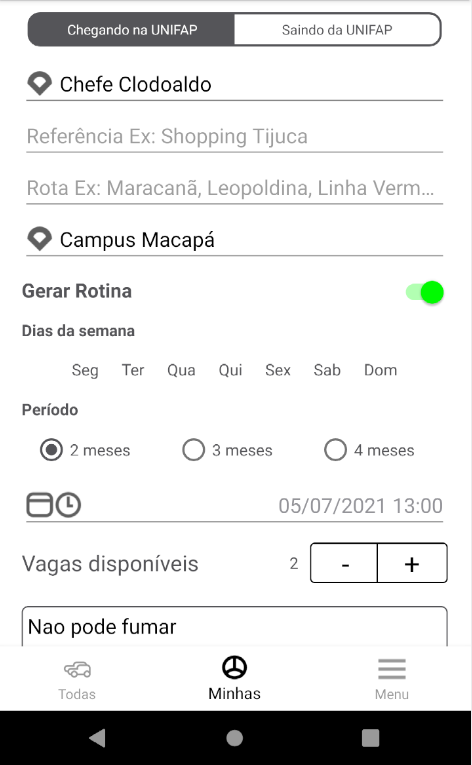
\includegraphics[width=0.29\textwidth]{./04-figuras/caronae/criacao_da_carona_carona_ufrj.png}
	\label{fig:publicar_carona}
	\fonte{Elaborada pelo autor} %acesso: 13/04/2021 
\end{figure}

O aplicativo exige que o usuário nas viagens de ida até a UFRJ tenha como ponto inicial algum bairro de uma das zonas cadastradas no sistema e como destino algum dos pontos/hubs da UFRJ. Nas viagens de volta é o contrário. Com capacidade de oferecer várias viagens durante o ano letivo, os criadores desenvolveram uma funcionalidade que permitisse os motoristas de agendar caronas futuras sem a necessidade de anunciar diariamente as caronas, característica automática que diferencia o Caronaê de outros pontos geradores de viagens (PGV) semelhantes.

Na lista disponibilizada no aplicativo, o usuário pode escolher entre as caronas ofertadas, ver detalhes sobre o trajeto e motorista, e caso lhe agrade, solicitar a carona. Já o motorista que ofereceu a carona pode aceitar ou não e acessar informações do caronista, caso aceite a corrida, um alerta é enviado para o caronista. O aplicativo também fornece aos envolvidos na corrida, um chat, informações adicionais como placa, cor do carro e modelo. A figura \ref{fig:solicitacao_de_carona} mostra a tela de solicitação de carona com a origem de um bairro da cidade e o destino o Campus Macapá.

\begin{figure}[!hbtp]
	\centering
	\caption{Notificação: Solicitação de Carona}
	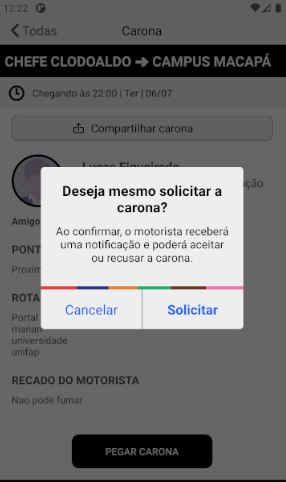
\includegraphics[width=0.29\textwidth]{./04-figuras/caronae/tela_solicitacao_de_carona_2.png}
	\label{fig:solicitacao_de_carona}
	\fonte{Elaborada pelo autor} %acesso: 13/04/2021 
\end{figure}

O "Meu Perfil" é possível ver as informações do usuário, se for o motorista, aparece as informações do veículo, número de caronas ofertadas e recebidas, no "Histórico", o usuário motorista consegue acompanhar quantas caronas foram concluídas ou quantas estão pendentes, e o caronista consegue ver quantas caronas pegou. Além disso, o sistema tem o "Falaê", onde os usuários pode manifestar suas sugestões ou críticas, e antes de tudo, o usuário precisa aceitar os termos de uso que também consta no aplicativo. Podemos ver isso na figura \ref{fig:telas_caronae}. 

\begin{figure}[!hbtp]
	\centering
	\caption{Telas do aplicativo Caronaê: login, busca e detalhe da carona}
	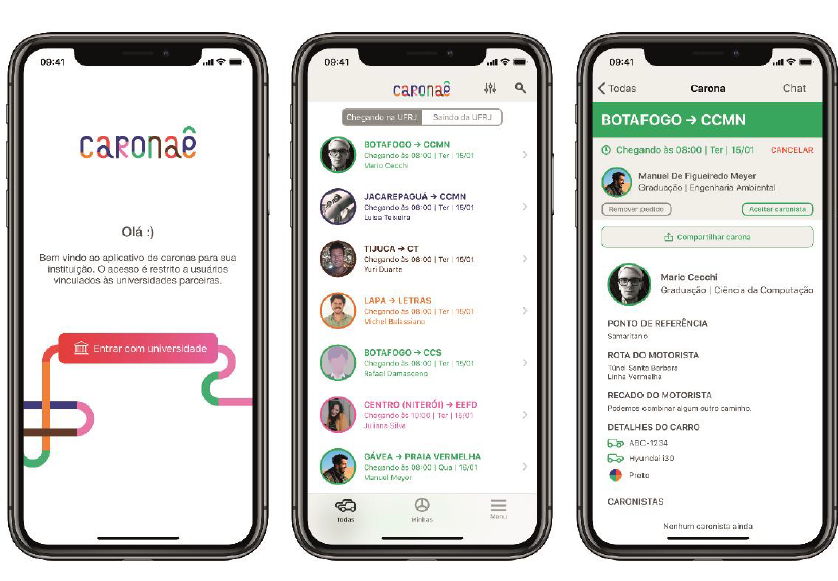
\includegraphics[width=0.5\textwidth]{./04-figuras/caronae-img-artigo.png}
	\label{fig:telas_caronae}
	\fonte{\cite{caronae}}
\end{figure}


Como plataforma digital, o caronaê possui um banco de dados onde registra todas as informações e interações dos serviços. O banco de dados do Caronaê é PostgreSQL, banco de dados objeto-relacionado acessado pela ferramenta administradora PGAdmin4 \footnote{https://www.pgadmin.org/}. O projeto também possuí uma área administrativa contruída com o framework laravel, onde os administradores tem acesso aos dados gerados na aplicação sem precisar realizar a consulta diretamente ao banco, o que exigiria conhecimento da linguagem SQL. \footnote{\textit{StructureStructure Query Language}: é a linguagem de pesquisa declarativa padrão para banco de dados relacional.} 

O sistema inicialmente era hospedado nos servidores da UFRJ, estando exposto a qualquer tipo de instabilidade. Após expandir e ter vários acessos simultâneos, a hospedagem da universidade já não supria a demanda, e os responsáveis pelo projeto começaram a ter problemas de disponibilidade por conta da infraestrutura. Para manter o sistema em funcionamento, a solução foi migrar todo o serviço próprio do Caronaê (backend, sistema administrativo, sistema intermediário de autenticação) para a "nuvem", utilizando a IaaS da empresa Amazon por 3 anos, entre os anos de 2016 e 2019. Após esse período o projeto foi descontinuado \cite{caronae}. 

Para finalizar o resumo das características da solução, o Caronaê, pensando na segurança do usuário, garante o acesso somente à comunidade acadêmica, para garantir isso, o aplicativo se conecta à base de dados da UFRJ através do sistema de gestão, onde busca os dados do aluno no SIGA(nome, curso, foto, se é Servidor, se está na Graduação, Mestrado). O acesso se dá pelo CPF e senha do usuário ativo na UFRJ. Segundo \cite{caronae}, durante o desenvolvimento da pesquisa, essa premissa resultou na criação de um portal específico na Intranet da UFRJ, especifico para os registros do serviço, nele constava todas informações dos usuários, como por exemplo, faixa etária e gênero, essas informações, segundo ela era relevante, a ausência dificultava nas consultas.

Os serviços utilizados para a autenticação dos usuários são \footnote{Disponível em: https://github.com/caronae/caronae-ufrj-authentication. Acesso: 06 Jun. 2021}:

\begin{itemize}
   

 \item \textbf{phpCas:} biblioteca que faz a integração com o CAS (Central Authentication Service) da Intranet UFRJ, que valida que o usuário é vinculado à UFRJ

 \item \textbf{SigaService:} comunica com o SIGA UFRJ, de onde são buscados os dados dos usuários 

 \item \textbf{CaronaeService:} parte do caronae-sdk-php \footnote{Disponivel em: https://github.com/caronae/caronae-sdk-php. Acesso em: 06 Jun. 2021}, é a classe que faz a comunicação com a API do Caronaê e é usada para enviar os dados do usuário para o Caronaê

 \item \textbf{CaronaeSigaAdaptor:} faz a conversão dos dados no formato que vem do SIGA para o formato da API do Caronaê

 \item \textbf{CaronaeUFRJAgent:} faz o fluxo de autenticação e autorização integrando todos os serviços acima
\end{itemize}


\begin{figure}[!hbtp]
	\centering
	\caption{Fluxograma da autenticação do Caronaê}
	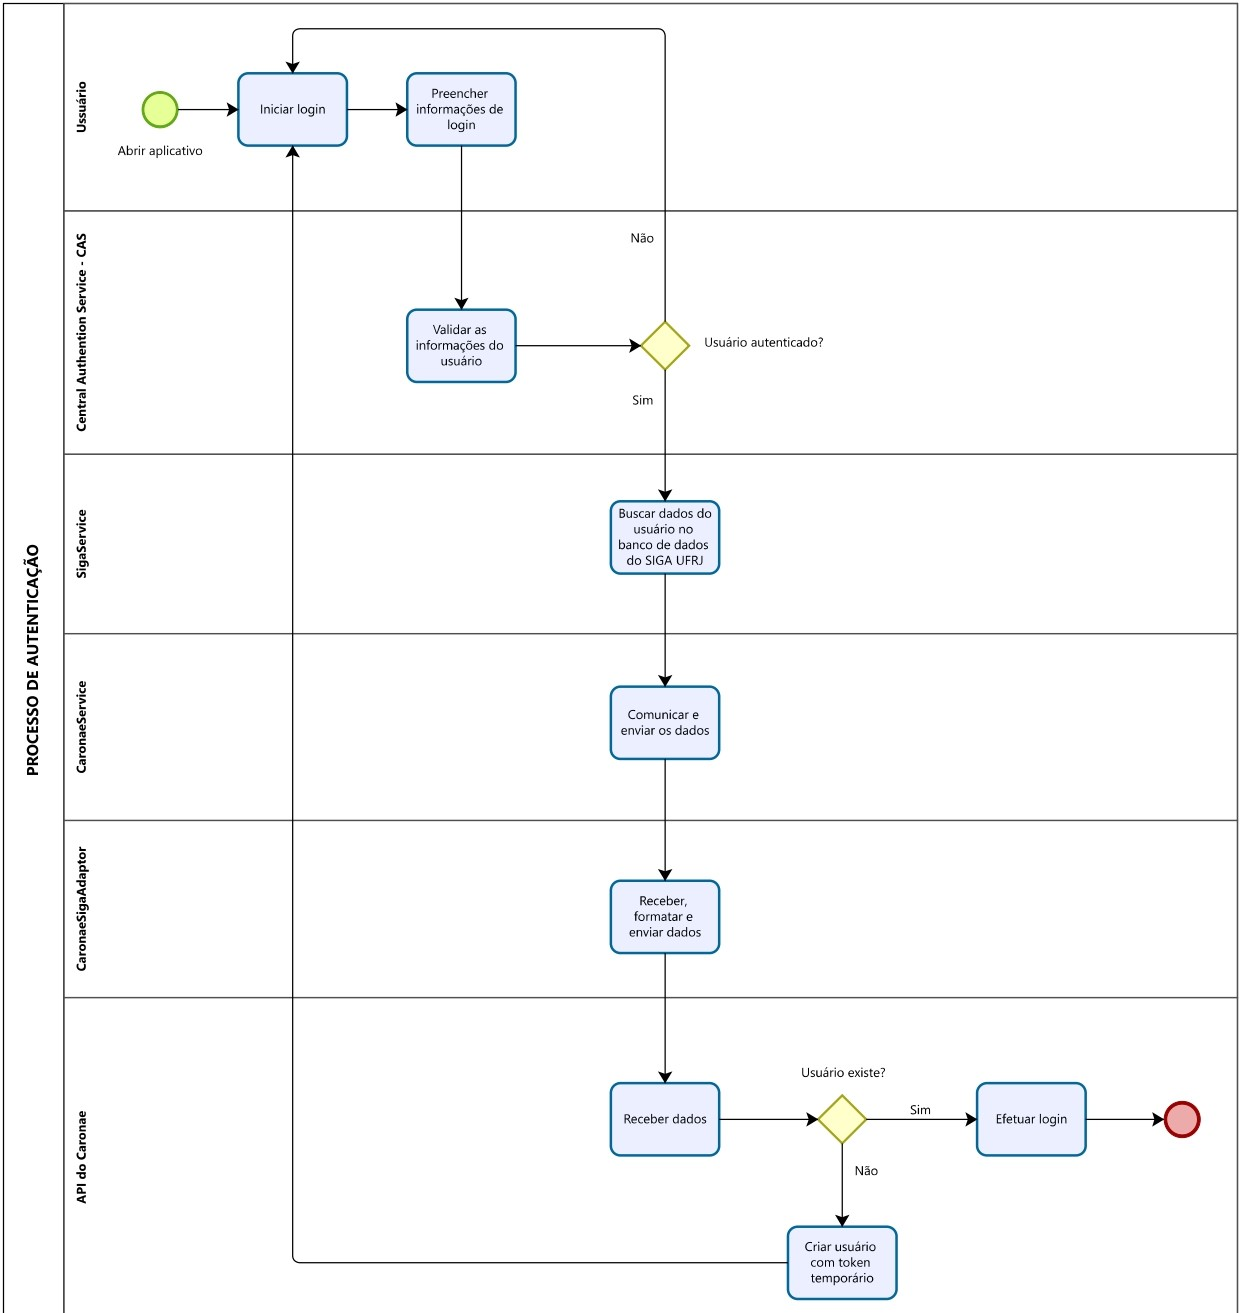
\includegraphics[width=0.6\textwidth]{./04-figuras/caronae/diagrama_bizagi.jpg}
	\label{fig:fluxograma}
	\fonte{Elaborada pelo autor.}
\end{figure}



\begin{comment}
%
	\mnote{Patrícia: falar sobre as características do Caronaê para a UFRJ, as que foram levantadas na análise de requisitos deles e que foram implementadas.}
    % Comentado só para sumir o texto do lado do documento
\end{comment}

\subsection{Características do Caronaê para UNIFAP}

Inicialmente, as mudanças realizadas para o aplicativo se adequar com a realidade dos usuários da UNIFAP foi alterar as zonas e bairros que se encontram no site da prefeitura de Macapá \footnote{https://macapa.ap.gov.br/portal/wp-content/uploads/2020/11/DIVISAO-POR-TERRITORIOS.pdf}, informando a zona e quais bairros pertencem aquela zona. Outras mudanças realizadas foram as alterações de campos que aparecem UFRJ para UNIFAP, na figura \ref{fig:carona_ate_a_unifap} mostra o bairro selecionado na tela do aplicativo.

\begin{figure}[!hbtp]
	\centering
	\caption{Tela de criação de carona: Chegando na Unifap}
	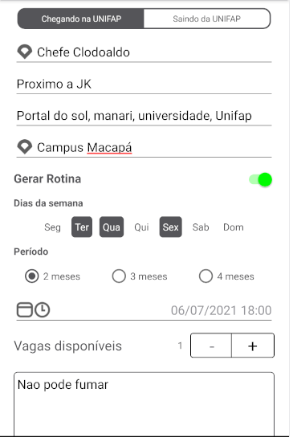
\includegraphics[width=0.17\textwidth]{./04-figuras/caronae/tela_criacao_da_carona_de_chegada_na_unifap.png}
	\label{fig:carona_ate_a_unifap}
	\fonte{Elaborada pelo autor.}
\end{figure}

Pontos de encontro ou Hubs, no qual ajuda os motoristas e caroneiros a se encontrarem também foram adicionados no sistema, levamos em consideração os departamentos da UNIFAP, DCET, DED, DEAD, DFCH, DEMAD, DEPLA, DCBS, Reitoria. Na figura \ref{fig:carona_saindo_da_unifap} podemos ver o cadastro da carona saindo da unifap, onde semelhante a carona chegando a Unifap selecionamos o bairro de saída e chega, uma referência da localização os bairros por onde vai passar com uma diferença, na saída da Unifap, o usuário precisa selecionar o ponto de encontro.

\begin{figure}[!hbtp]
	\centering
	\caption{Tela da criação de carona: Saindo da Unifap}
	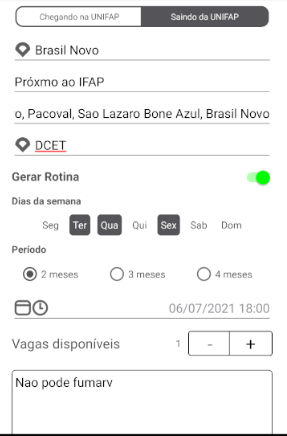
\includegraphics[width=0.25\textwidth]{./04-figuras/caronae/tela_criacao_da_carona_de_saida_da_unifapp.png}
	\label{fig:carona_saindo_da_unifap}
	\fonte{Elaborada pelo autor.}
\end{figure}

Além destes pontos mencionados, o Caronaê para a Universidade também tem como característica o acesso apenas por pessoas ligadas a Unifap, porém, diferente da UFRJ, não temos uma solução que disponibilize os dados dos alunos, professores e técnicos para a solução consumir. Na figura \ref{fig:tela_usuarios_painel_administrativo} mostra o painel administrativo do Caronaê, onde é gerenciado usuários, caronas, zonas e bairros, administradores instituições, onde é possível bloquear usuários caso seja necessário, entre outras funções, na figura podemos ver alguns nomes de usuários e informações que foram geradas em um banco de dados fictício, mas que em produção utiliza de serviços para consumir da base de dados real da universidade.

\begin{figure}[!hbtp]
	\centering
	\caption{Tela da criação de carona: Saindo da Unifap}
	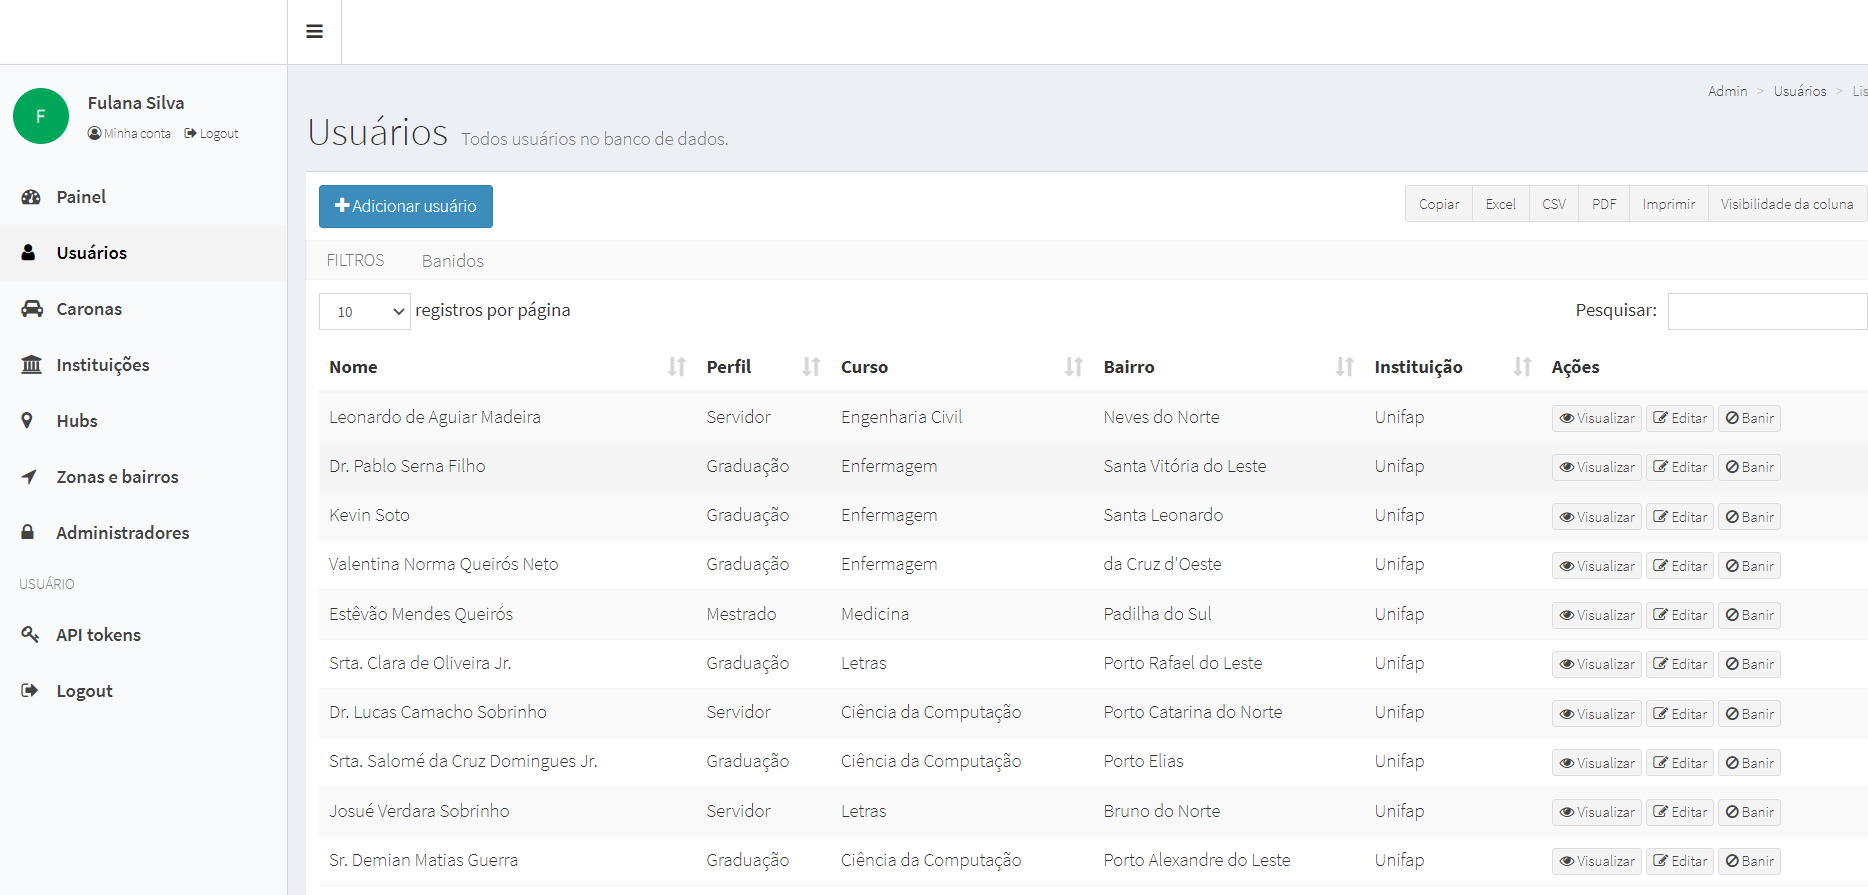
\includegraphics[width=0.9\textwidth]{./04-figuras/caronae/tela_usuarios_do_painel_administrativo.png}
	\label{fig:tela_usuarios_painel_administrativo}
	\fonte{Elaborada pelo autor.}
\end{figure}

No momento, para utilizar o aplicativo estão rodando em um banco de dados PostgreSQL \footnote{https://www.postgresql.org/docs/} local, o serviço de backend e do sistema administrativo pelo servidor local do laravel \footnote{https://laravel.com/} e o emulador do Android Studio\footnote{https://developer.android.com/studio} também localmente.

\begin{comment}
	\mnote{Patrícia: falar sobre que características o Caronaê deveria ter para ser implementado na UNIFAP, que características já existentes permaneceriam, que características já existentes devem ser adaptadas ou modificadas, que características já existentes devem ser retiradas e que características devem ser incluídas considerando o contexto da Unifap e Macapá. Isso seria o seu levantamento de requisitos.}
\end{comment}


\begin{comment}

\subsection{Dificuldades Enfrentadas}

As dificuldades iniciais foi a de tentar executar todos os serviços presentes na aplicação, todos os microserviços de aunteticação e notificação do aplicativo, porém, isso não se deu porque a API que auxiliava o projeto, API está, fornecidade pela universidade não está mais online.

Outros microserviços dependem do funcionamento e do acesso as APIs que UFRJ disponibilizava, entretanto, foi deixado de lado essas tentativas e focado apenas na execução local, com banco de dados local, API apenas do Caronaê com dados de alguns usuários que estão cadastrados nas querys do projeto e o no funcionamento do API e integração dos serviços. O fato de não termos uma API na universidade onde eu possa testar a aplicação também dificulta a proposta, claro que antes algumas coisas precisariam ser avaliadas, como o tratamento dos dados do SIGAA UNIFAP para o formato que a API do Caronaê recebe, caso fosse necessário.

\end{comment}

\begin{comment}
\section{Próximos passos}
Será funcionar o aplicativo junto ao back-end da aplicação seja ele utilizando as imagens do docker ou utilizando outros serviços similares aos utilizados, como o XAMPP que oferecem os serviços Apache como servidor Web, Mysql como banco de dados e PHP.

Ainda incluindo também uma forma ou opção de como consumir as informações do sistema de gestão da Unifap, algo que pode ser visto mais a frente quando os primeiros passos forem realizados, objetivo contudo é apresentar e mostrar que o código fonte pode ser reaproveitado e dado continuidade numa ideia interessante realizada pela equipe Caronaê.
\end{comment}

